\section{Metodi numerici}

%-----------------------------------------%
%				Prima slide				  %
%	        Metropolis vs Wolff     	  %
%-----------------------------------------%
\begin{frame}
    \frametitle{Metropolis vs Wolff}
    \framesubtitle{}

    \begin{columns}

        \begin{column}{0.5\textwidth}
            \begin{block}{Metropolis}

                \begin{itemize}[itemsep=0.5em, label=$\diamond$]
                    \item Tentata inversione di un singolo spin
                    \item $A\left(\nu\,|\,\mu\right)\,=\,\text{min}\left[1,\,e^{-\beta\left(E_{\nu}\,-\,E_{\mu}\right)}\right]$
                    \item Ottimo per $T \ll T_c$ oppure $T \gg T_c$
                \end{itemize}

                \centering
                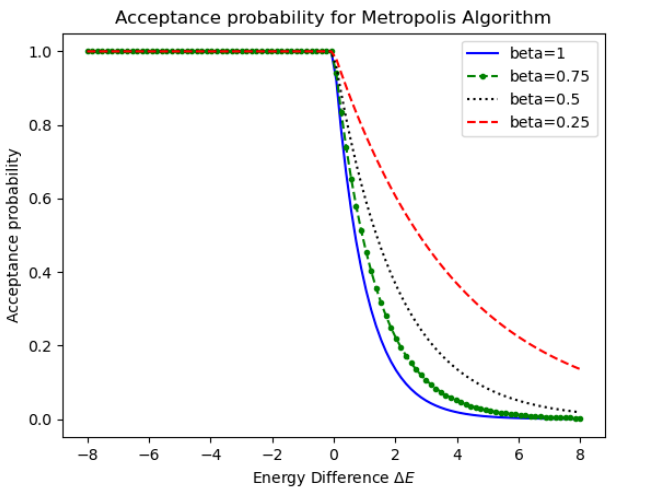
\includegraphics[width=0.7\textwidth]{Immagini/metodiNumerici/accRate_metro.png}	
                
            \end{block}
        \end{column}


        \begin{column}{0.5\textwidth}
            \begin{block}{Wolff}

                \begin{itemize}[itemsep=0.5em, label=$\diamond$]
                    \item Algoritmo di clustering
                    \item $P_{add}\,=\,1\,-\,\exp{\left(-2\beta J\right)}$
                    \item Ottimo per $T \simeq T_c$
                \end{itemize}

                \centering
                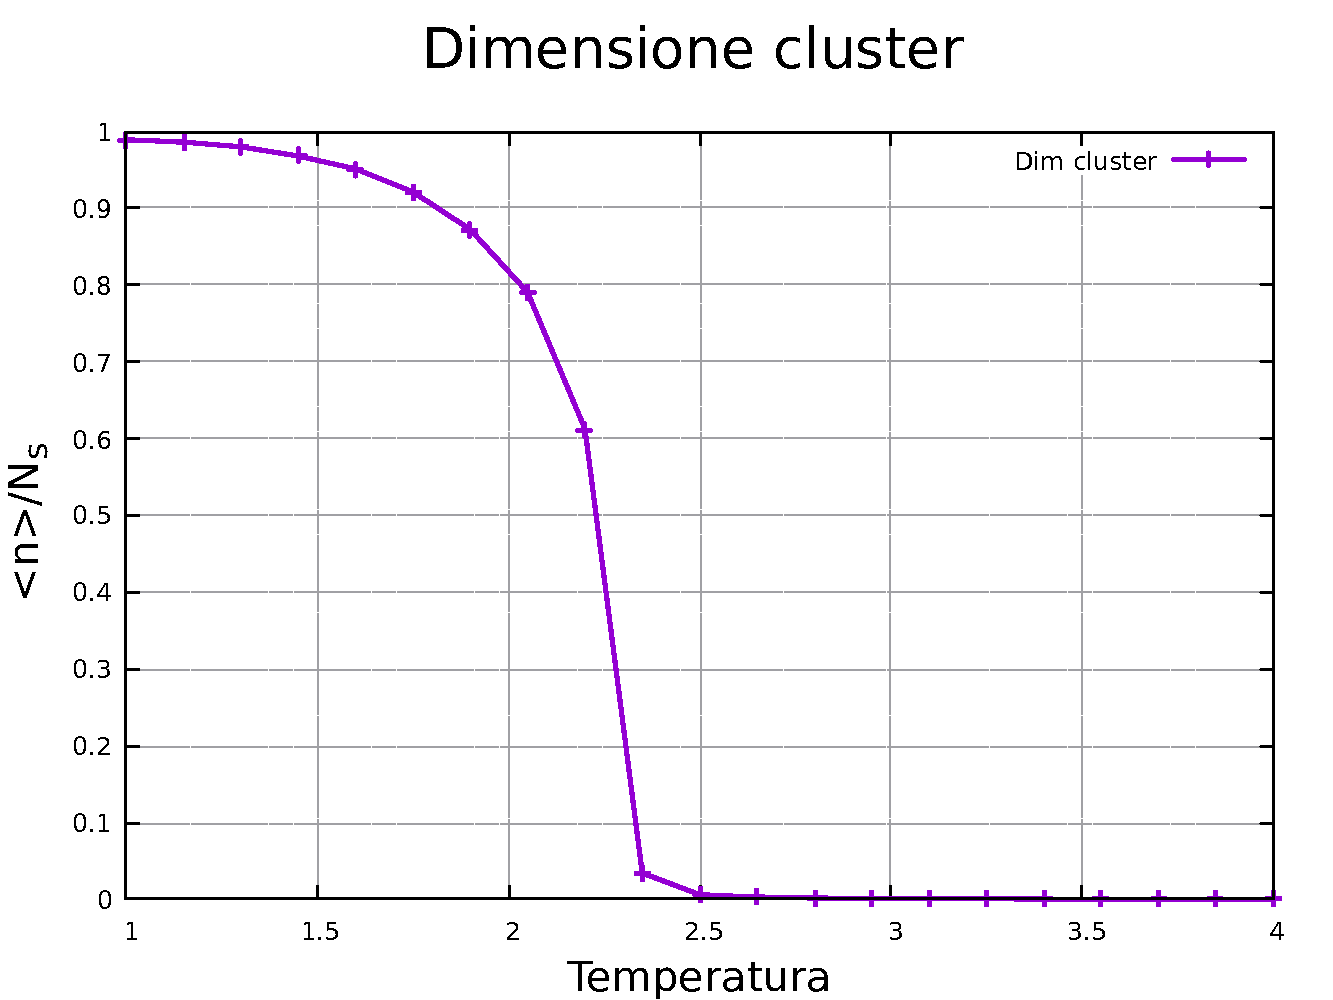
\includegraphics[width=0.7\textwidth]{Immagini/metodiNumerici/dimClFlip.pdf}			
            
            \end{block}
        \end{column}
      \end{columns}
  
\end{frame}


%-----------------------------------------%
%		       Seconda slide		      %
%       Termalizzazione del modello       %
%-----------------------------------------%
\begin{frame}
    \frametitle{Termalizzazione}
    \framesubtitle{}

    \begin{columns}

        \begin{column}{0.6\textwidth}

            \centering
            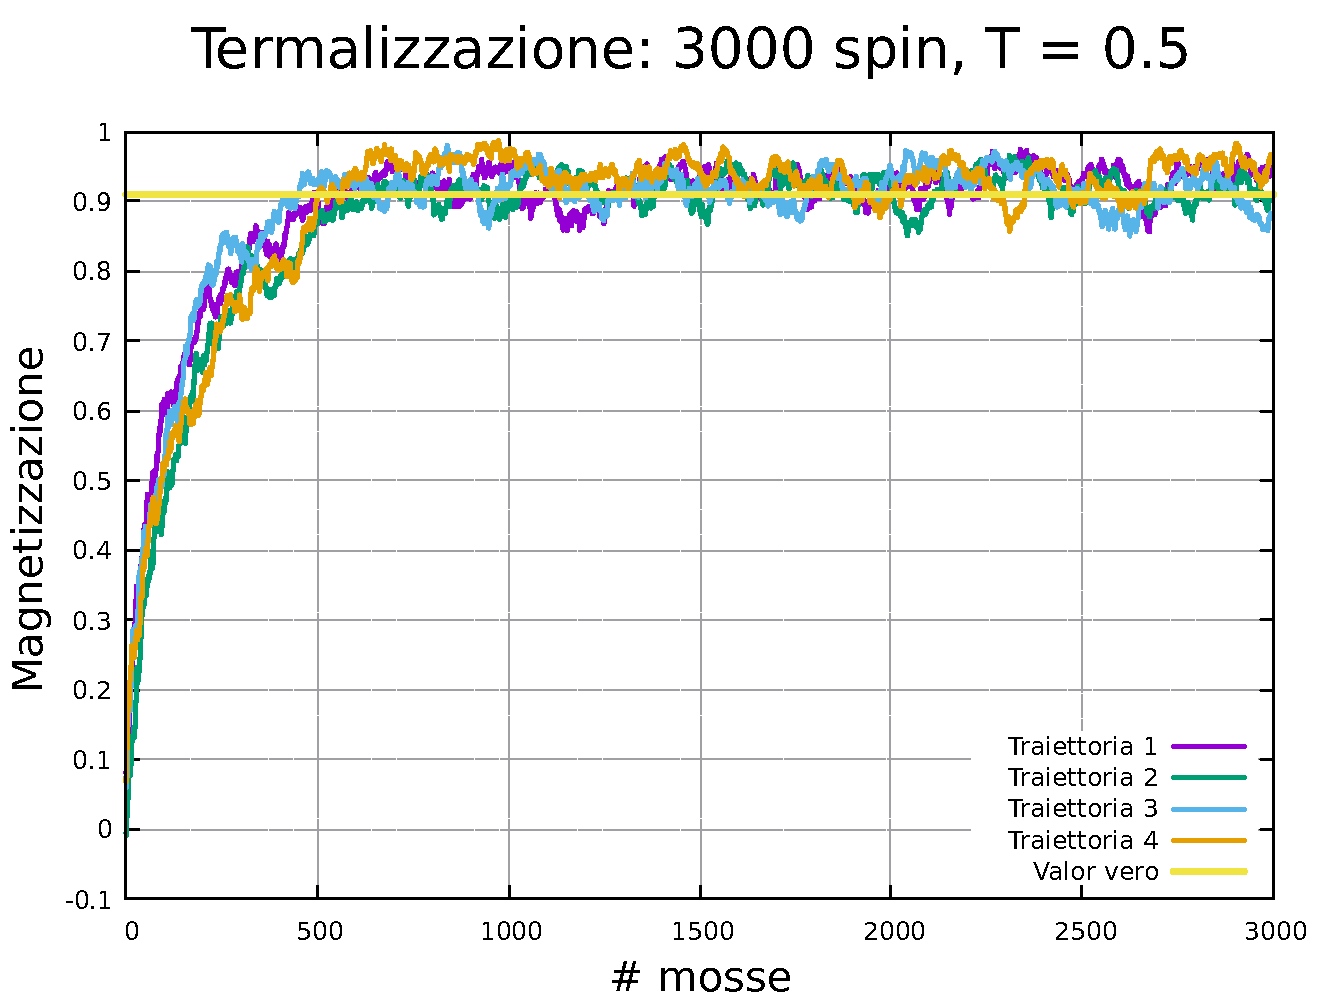
\includegraphics[width=\textwidth]{Immagini/metodiNumerici/term_3000_0.5.pdf}
            \newline
            {\scriptsize Termalizzazione per modello di Ising 1D.}

        \end{column}


        \begin{column}{0.4\textwidth}

            \begin{itemize}[itemsep=0.5em, label=$\diamond$]
                \item Giungere all'equilibrio termodinamico
                \item Attenzione a stati metastabili
                \item Dipendenza dalla condizione iniziale
            \end{itemize}
            
        \end{column}
      \end{columns}
  
\end{frame}
